\documentclass[letterpaper,oneside]{scrbook}
\usepackage{listings}
\usepackage{color}
\usepackage{tabularx}
\usepackage{graphicx}
\usepackage{hyperref}

\definecolor{codegreen}{rgb}{0,0.6,0}
\definecolor{codegray}{rgb}{0.5,0.5,0.5}
\definecolor{codepurple}{rgb}{0.58,0,0.82}
\definecolor{backcolour}{rgb}{0.95,0.95,0.92}
 
\lstdefinestyle{mystyle}{
    backgroundcolor=\color{backcolour},   
    commentstyle=\color{codegreen},
    keywordstyle=\color{magenta},
    numberstyle=\tiny\color{codegray},
    stringstyle=\color{codepurple},
    basicstyle=\normalsize\ttfamily,
    breakatwhitespace=false,         
    breaklines=true,                 
    captionpos=b,                    
    keepspaces=true,                 
    numbers=none,                    
    numbersep=5pt,                  
    showspaces=false,                
    showstringspaces=false,
    showtabs=false,                  
    tabsize=2
}
 
\lstset{style=mystyle}

\title{WVU High Performance Computing Seminars}
\author{Guillermo Avendano-Franco}

\begin{document}
%\maketitle
%\tableofcontents

\newpage
\begin{center}
\LARGE Schedule
\end{center}

\begin{tabularx}{0.95\textwidth}{|l|X|}
  \hline
  \multicolumn{2}{|c|}{Day 1 - June 12, 2017} \\
  \hline
09:00 - 10:00 & Login into remote systems (SSH, PuTTY and tmux)\\
10:00 - 11:00 & Command Line Interface\\
11:00 - 12:00 & Text Editors (nano, emacs and vi)\\
&\\
12:00 - 13:00 & Lunch Break\\
&\\
13:00 - 13:30 & Using Environmental Modules (module)\\
13:30 - 15:30 & Torque and Moab (qsub, qstat, qdel, checkjob)\\
15:30 - 16:00 & Transfering files (rsync and globus)\\
\hline
\end{tabularx}

\bigskip

\begin{tabularx}{0.95\textwidth}{|l|X|}
  \hline
  \multicolumn{2}{|c|}{Day 2 - June 13, 2017} \\
  \hline
09:00 - 10:00 & Shell Scripting (including grep)\\
10:00 - 11:00 & Python Scripting\\
11:00 - 12:00 & Using pip and virtualenv\\
&\\
12:00 - 13:00 & Lunch Break\\
&\\
13:00 - 14:00 & Plotting (gnuplot and matplotlib)\\
14:00 - 15:00 & Building Software (example with fftw)\\
15:00 - 16:00 & Creating Environmental Modules\\
\hline
\end{tabularx}

\bigskip

\begin{tabularx}{0.95\textwidth}{|l|X|}
  \hline
  \multicolumn{2}{|c|}{Day 3 - June 14, 2017} \\
  \hline
09:00 - 10:00 & Advanced Scripting (regular expressions)\\
10:00 - 11:00 & Programming in C, Fortran and Python I\\
11:00 - 12:00 & Programming in C, Fortran and Python II\\
&\\
12:00 - 13:00 & Lunch Break\\
&\\
13:00 - 14:00 & Parallel Programming (OpenMP)\\
14:00 - 15:00 & Parallel Programming (MPI)\\
15:00 - 15:30 & Test Driven Development (Python nose)\\
15:30 - 16:00 & Version Control with Git\\
\hline
\end{tabularx}

%\chapter{Linux, Command Line and HPC Environment (Newcomer)}


\section{Logging into remote systems}

Currently WVU has two clusters for HPC, mountaineer and spruce. You can access them using SSH.
SSH provides a secure channel over an unsecured network such as internet.
Both Linux and macOS commonly include the SSH client by default. On Windows machines you can use a free application called PuTTY.

To connect to Mountaineer use:

\begin{lstlisting}[language=bash]
ssh <username>@mountaineer.hpc.wvu.edu
\end{lstlisting}

For Spruce

\begin{lstlisting}[language=bash]
ssh <username>@spruce.hpc.wvu.edu
\end{lstlisting}

Once you enter on the system, you can start typing commands. You can open several connections simultaneously. Each connection is independent of each other.

Power users can benefit from a terminal multiplexer such as tmux. tmux allows users to keep several virtual windows and panels open from a single connection. It offers also preserve the terminal status in case of disconnection from the server.

To use tmux, first connect to the server and execute the command

\begin{lstlisting}[language=bash]
tmux
\end{lstlisting}

You can create new virtual windows with \texttt{CTRL-b c}, you move between windows with \texttt{CTRL-b n} and \texttt{CTRL-b p}. You can detach from your multiplexed terminals with \texttt{CTRL-b d}. 

If for some reason you lost the connection to the server or you detached from the mulpiplexer all that you have to do to reconnect is to execute the command:

\begin{lstlisting}[language=bash]
tmux a
\end{lstlisting}

There are many options for using tmux, see the cheat cheat for some of them.

\section{Top 10 commands to learn}

When you interact with a HPC cluster your interaction is basically by executing commands on a terminal and editing text files. For newcomers using command lines could be a frustrating experience knowing that there are literally hundreds of commands. Certainly there are manuals for most of those commands, but they are of no use if you do not know which is the command you need to use for each situation. The good news is that you can do a lot of things with just a bunch of them and you can learn others in due time.

This is a selection of the 10 most essential commands you need to learn.

\subsection{ls}

List all the files in a directory. Linux as many Operating Systems organize files in files and directories (also called folders). 

\begin{lstlisting}[language=bash]
$ ls
file0a  file0b  folder1  folder2 link0a  link2a
\end{lstlisting}

Some terminal offer color output so you can differentiate normal files from folders. You can make the difference more clear with this

\begin{lstlisting}[language=bash]
$ ls -aCF
./  ../  file0a  file0b  folder1/  folder2/ link0a@  link2a@
\end{lstlisting}

You will see a two extra directories \texttt{"."} and \texttt{".."}. Those are special folders that refer to the current folder and the folder up in the tree.
Directories have the suffix \texttt{"/"}. Symbolic links, kind of shortcuts to other files or directories are indicated with the symbol \texttt{"@"}.

Another option to get more information about the files in the system is:

\begin{lstlisting}[language=bash]
$ ls -al
total 36
drwxrwxr-x.  4 gufranco users     86 May 30 12:16 .
drwxr-xr-x. 82 gufranco users  12288 May 30 12:05 ..
-rw-rw-r--.  1 gufranco users      0 May 30 12:08 file0a
-rw-rw-r--.  1 gufranco users      0 May 30 12:08 file0b
drwxrwxr-x.  2 gufranco users     32 May 30 12:07 folder1
drwxrwxr-x.  2 gufranco users     32 May 30 12:07 folder2
lrwxrwxrwx.  1 gufranco users      6 May 30 12:16 link0a -> file0a
lrwxrwxrwx.  1 gufranco users     14 May 30 12:16 link2a -> folder2/file2a
\end{lstlisting}

Those characters on the first column indicate the permissions. The first character will be "d" for directories, "l" for symbolic links and "-" for normal files. The next 3 characters are the permissions for "read", "write" and "execute" for the owner. The next 3 are for the group, and the final 3 are for others.
The meaning of "execute" for a file indicates that the file could be a script or binary executable. For a directory it means that you can see its contents. 

\subsection{cp}

This command copies the contents of one file into another file. For example

\begin{lstlisting}[language=bash]
$ cp file0b file0c
\end{lstlisting}

\subsection{rm}

This command deletes the contents of one file. For example

\begin{lstlisting}[language=bash]
$ rm file0c
\end{lstlisting}

There is no such thing like a trash folder on a HPC system. Deleting a file should be consider an irreversible operation.

Recursive deletes can be done with

\begin{lstlisting}[language=bash]
$ rm -rf folder_to_delete
\end{lstlisting}

Be extremely cautious deleting files recursively. You cannot damage the system as the files that you do not own you cannot delete. However, you can delete all your files forever.

\subsection{mv}

This command moves a files from one directory to another. It also can be used to rename files or directories.

\begin{lstlisting}[language=bash]
$ mv file0b file0c
\end{lstlisting}

\subsection{pwd}

It is easy to get lost when you move in complex directory structures. pwd will tell you the current directory.

\begin{lstlisting}[language=bash]
$ pwd
/home/gufranco/Dropbox/SummerHandsOn
\end{lstlisting}

\subsection{cd}

This command moves you to the directory indicated as an argument, if no argument is given, it returns to your home directory.

\begin{lstlisting}[language=bash]
$ cd folder1
\end{lstlisting}

\subsection{cat and tac}

When you want to see the contents of a text file, the command cat displays the contents on the screen. It is also useful when you want to concatenate the contents of several files.

\begin{lstlisting}[language=bash]
$ cat INCAR 
system   =  LiAu
PREC      =  High
NELMIN    =  8
NELM      =  100
EDIFF     =  1E-07
...
\end{lstlisting}

To concatenate files you need to use the symbol \texttt{">"} indicating that you want to redirect the output of a command into a file

\begin{lstlisting}[language=bash]
$ cat file1 file2 file3 > file_all
\end{lstlisting}

The command tac shows the files in reverse starting from the last line back to the first one.

\subsection{more and less}

Sometimes text files, as those created as product of simulations are too large to be seen in one screen, the command "more" shows the files one screen at a time. The command \texttt{"less"} offers more functionality and should be the tool of choice to see large text files. 

\begin{lstlisting}[language=bash]
$ less OUTCAR
\end{lstlisting}

\subsection{ln}

This command allow to create links between files. Used wisely could help you save time when traveling frequently to deep directories. By default it creates hard links. Hard links are like copies, but they make references to the same place in disk. Symbolic links are better in many cases because you can cross file systems and partitions. To create a symbolic link

\begin{lstlisting}[language=bash]
$ ln -s file1 link_to_file1
\end{lstlisting}
 
\subsection{grep}

The grep command extract from its input the lines containing a specified string or regular expression. It is a powerful command for extracting specific information from large files. Consider for example

\begin{lstlisting}[language=bash]
$ grep TOTEN OUTCAR
  free energy    TOTEN  =        68.29101273 eV
  free energy    TOTEN  =       -13.46870926 eV
  free energy    TOTEN  =       -18.78141268 eV
  ...
\end{lstlisting}
  
Regular expressions offers ways to specified text strings that could vary in several ways and allow commands such as grep to extract those strings efficiently. We will see more about regular expressions in third chapter.

\subsection{More commands}

The 10 commands above, will give you enough tools to move files around and travel the directory tree. There are more commands summarized 

\begin{tabularx}{0.75\textwidth}{|l|X|}
\hline
\multicolumn{2}{|c|}{Output of entire files}\\ \hline
cat  &                Concatenate and write files\\
tac  &                Concatenate and write files in reverse\\
nl  &                 Number lines and write files\\
od  &                 Write files in octal or other formats\\
base64  &             Transform data into printable data\\
\hline
\end{tabularx}

\begin{tabularx}{0.75\textwidth}{|l|X|}
\hline
\multicolumn{2}{|c|}{Formatting file contents}\\ \hline
fmt  &                Reformat paragraph text\\
numfmt  &             Reformat numbers\\
pr  &                 Paginate or columnate files for printing\\
fold  &               Wrap input lines to fit in specified width\\
\hline
\end{tabularx}

\begin{tabularx}{0.75\textwidth}{|l|X|}
\hline
\multicolumn{2}{|c|}{Output of parts of files}\\ \hline
head  &               Output the first part of files\\
tail  &               Output the last part of files\\
split  &              Split a file into fixed-size pieces\\
csplit  &             Split a file into context-determined pieces\\
\hline
\end{tabularx}

\begin{tabularx}{0.75\textwidth}{|l|X|}
\hline
\multicolumn{2}{|c|}{Summarizing files}\\ \hline
wc  &                 Print newline, word, and byte counts\\
sum  &                Print checksum and block counts\\
cksum  &              Print CRC checksum and byte counts\\
md5sum  &             Print or check MD5 digests\\
sha1sum  &            Print or check SHA-1 digests\\
sha2 utilities &                Print or check SHA-2 digests\\
\hline
\end{tabularx}

\begin{tabularx}{0.75\textwidth}{|l|X|}
\hline
\multicolumn{2}{|c|}{Operating on sorted files}\\ \hline
sort  &               Sort text files\\
shuf  &               Shuffle text files\\
uniq  &               Uniquify files\\
comm  &               Compare two sorted files line by line\\
ptx  &                Produce a permuted index of file contents\\
tsort  &              Topological sort\\
\hline
\end{tabularx}

\begin{tabularx}{0.75\textwidth}{|l|X|}
\hline
\multicolumn{2}{|c|}{Operating on fields}\\ \hline
cut  &                Print selected parts of lines\\
paste  &              Merge lines of files\\
join  &               Join lines on a common field\\
\hline
\end{tabularx}

\begin{tabularx}{0.75\textwidth}{|l|X|}
\hline
\multicolumn{2}{|c|}{Operating on characters}\\ \hline
tr  &                 Translate, squeeze, and/or delete characters\\
expand  &             Convert tabs to spaces\\
unexpand  &           Convert spaces to tabs\\
\hline
\end{tabularx}

\begin{tabularx}{0.75\textwidth}{|l|X|}
\hline
\multicolumn{2}{|c|}{Directory listing}\\ \hline
ls  &                 List directory contents\\
dir  &                Briefly list directory contents\\
vdir  &               Verbosely list directory contents\\
dircolors  &          Color setup for 'ls'\\
\hline
\end{tabularx}

\begin{tabularx}{0.75\textwidth}{|l|X|}
\hline
\multicolumn{2}{|c|}{Basic operations}\\ \hline
cp  &                 Copy files and directories\\
dd  &                 Convert and copy a file\\
install  &            Copy files and set attributes\\
mv  &                 Move (rename) files\\
rm  &                 Remove files or directories\\
shred  &              Remove files more securely\\
\hline
\end{tabularx}

\begin{tabularx}{0.75\textwidth}{|l|X|}
\hline
\multicolumn{2}{|c|}{Special file types}\\ \hline
link  &               Make a hard link via the link syscall\\
ln  &                 Make links between files\\
mkdir  &              Make directories\\
mkfifo  &             Make FIFOs (named pipes)\\
mknod  &              Make block or character special files\\
readlink  &           Print value of a symlink or canonical file name\\
rmdir  &              Remove empty directories\\
unlink  &             Remove files via unlink syscall\\
\hline
\end{tabularx}

\begin{tabularx}{0.75\textwidth}{|l|X|}
\hline
\multicolumn{2}{|c|}{Changing file attributes}\\ \hline
chown  &              Change file owner and group\\
chgrp  &              Change group ownership\\
chmod  &              Change access permissions\\
touch  &              Change file timestamps\\
\hline
\end{tabularx}

\begin{tabularx}{0.75\textwidth}{|l|X|}
\hline
\multicolumn{2}{|c|}{Disk usage}\\ \hline
df  &                 Report file system disk space usage\\
du  &                 Estimate file space usage\\
stat  &               Report file or file system status\\
sync  &               Synchronize data on disk with memory\\
truncate  &           Shrink or extend the size of a file\\
\hline
\end{tabularx}

\begin{tabularx}{0.75\textwidth}{|l|X|}
\hline
\multicolumn{2}{|c|}{Printing text}\\ \hline
echo  &               Print a line of text\\
printf  &             Format and print data\\
yes  &                Print a string until interrupted\\
\hline
\end{tabularx}

\begin{tabularx}{0.75\textwidth}{|l|X|}
\hline
\multicolumn{2}{|c|}{Conditions}\\ \hline
false  &              Do nothing, unsuccessfully\\
true  &               Do nothing, successfully\\
test  &               Check file types and compare values\\
expr  &               Evaluate expressions\\
tee  &                Redirect output to multiple files or processes\\
\hline
\end{tabularx}

\begin{tabularx}{0.75\textwidth}{|l|X|}
\hline
\multicolumn{2}{|c|}{File name manipulation}\\ \hline
basename  &           Strip directory and suffix from a file name\\
dirname  &            Strip last file name component\\
pathchk  &            Check file name validity and portability\\
mktemp  &             Create temporary file or directory\\
realpath  &           Print resolved file names\\
\hline
\end{tabularx}

\begin{tabularx}{0.75\textwidth}{|l|X|}
\hline
\multicolumn{2}{|c|}{Working context}\\ \hline
pwd  &                Print working directory\\
stty  &               Print or change terminal characteristics\\
printenv  &           Print all or some environment variables\\
tty  &                Print file name of terminal on standard input\\
\hline
\end{tabularx}

\begin{tabularx}{0.75\textwidth}{|l|X|}
\hline
\multicolumn{2}{|c|}{User information}\\ \hline
id  &                 Print user identity\\
logname  &            Print current login name\\
whoami  &             Print effective user ID\\
groups  &             Print group names a user is in\\
users  &              Print login names of users currently logged in\\
who  &                Print who is currently logged in\\
\hline
\end{tabularx}

\begin{tabularx}{0.75\textwidth}{|l|X|}
\hline
\multicolumn{2}{|c|}{System context}\\ \hline
arch  &               Print machine hardware name\\
date  &               Print or set system date and time\\
nproc  &              Print the number of processors\\
uname  &              Print system information\\
hostname  &           Print or set system name\\
hostid  &             Print numeric host identifier\\
uptime  &             Print system uptime and load\\
\hline
\end{tabularx}

\begin{tabularx}{0.75\textwidth}{|l|X|}
\hline
\multicolumn{2}{|c|}{Modified command}\\ \hline
chroot  &             Run a command with a different root directory\\
env  &                Run a command in a modified environment\\
nice  &               Run a command with modified niceness\\
nohup  &              Run a command immune to hangups\\
stdbuf  &             Run a command with modified I/O buffering\\
timeout  &            Run a command with a time limit\\
\hline
\end{tabularx}

\begin{tabularx}{0.75\textwidth}{|l|X|}
\hline
\multicolumn{2}{|c|}{Process control}\\ \hline
kill  &               Sending a signal to processes\\
\hline
\end{tabularx}

\begin{tabularx}{0.75\textwidth}{|l|X|}
\hline
\multicolumn{2}{|c|}{Delaying}\\ \hline
sleep  &              Delay for a specified time\\
\hline
\end{tabularx}

\begin{tabularx}{0.75\textwidth}{|l|X|}
\hline
\multicolumn{2}{|c|}{Numeric operations}\\ \hline
factor  &             Print prime factors\\
seq  &                Print numeric sequences\\
\hline
\end{tabularx} 


\section{Text Editors}

There are several terminal-based editors available on our clusters. We will focus our attention to three of them: nano, emacs and vim. 
Your choice of an editor depends mostly on how much functionality do you want from your editor, how many fingers do you want to use for a given command and the learning curve to master it.
For HPC users the editor is an important choice. Most of your time you are on the terminal executing commands or editing files, being those input files, submission scripts or the output of your calculations.


Lets review those three editors to give you the opportunity to have an informative choice.

\subsection{Nano}

Nano is a small, free and friendly editor with commands that usually manage using the Control (CTRL) combined with some other key.

You can start editing a file using a command line like this

  nano myfile.f90

There are several commands available, the list below comes from the help text.
When you see the symbol \verb|"^"| it means to press the Control (CTRL) key, the symbol
\verb|"M-"| is called Meta, but in most keyboards is identified with the (Alt) key. 

\begin{lstlisting}
^G	(F1)            Display the help text
^X	(F2)            Close the current file buffer / Exit from nano
^O	(F3)            Write the current file to disk
^J	(F4)            Justify the current paragraph

^R	(F5)            Insert another file into the current one
^W	(F6)            Search for a string or a regular expression
^Y	(F7)            Move to the previous screen
^V	(F8)            Move to the next screen

^K	(F9)            Cut the current line and store it in the cutbuffer
^U	(F10)           Uncut from the cutbuffer into the current line
^C	(F11)           Display the position of the cursor
^T	(F12)           Invoke the spell checker, if available
\end{lstlisting}

The most basic usage is to edit a file, and exit from the editor with CTRL-X.
Nano ask you if you want to save the file, you answer "Y" and offers you a name.
Simply press ENTER and your file is saved.

\subsection{Emacs}

Emacs is an extensible, customizable, open-source text editor. Together with Vi/Vim is one the most widely
used editors in Linux environments. There are a big number of commands, customizations and extra modules 
that can be integrated with Emacs. We will just go briefly covering the basics.

The number of commands for Emacs is large, here the basic list of commands for editing, moving and searching text.

\subsubsection{Entering Emacs}

\begin{lstlisting}
 emacs <filename>
\end{lstlisting}

\subsubsection{Leaving Emacs}

\begin{lstlisting}
 suspend Emacs (or iconify it under X) C-z
 exit Emacs permanently C-x C-c
\end{lstlisting}

\subsubsection{Files}

\begin{lstlisting}
 read a file into Emacs C-x C-f
 save a file back to disk C-x C-s
 save all files C-x s
 insert contents of another file into this buffer C-x i
 replace this file with the file you really want C-x C-v
 write buffer to a specified file C-x C-w
 toggle read-only status of buffer C-x C-q
\end{lstlisting}

\subsubsection{Incremental Search}

\begin{lstlisting}
 search forward C-s
 search backward C-r
 regular expression search C-M-s
 reverse regular expression search C-M-r
 select previous search string M-p
 select next later search string M-n
 exit incremental search RET
 undo effect of last character DEL
 abort current search C-g
 Use C-s or C-r again to repeat the search in either direction. If
 Emacs is still searching, C-g cancels only the part not matched.
\end{lstlisting}

\subsubsection{Motion}

\begin{lstlisting}
 entity to move over backward forward
 character C-b C-f
 word M-b M-f
 line C-p C-n
 go to line beginning (or end) C-a C-e
 sentence M-a M-e
 paragraph M-{ M-}
 page C-x [ C-x ]
 sexp C-M-b C-M-f
 function C-M-a C-M-e
 go to buffer beginning (or end) M-< M->
 scroll to next screen C-v
 scroll to previous screen M-v
 scroll left C-x <
 scroll right C-x >
 scroll current line to center, top, bottom C-l
 goto line M-g g
 goto char M-g c
 back to indentation M-m
\end{lstlisting}

\subsubsection{Killing and Deleting}

\begin{lstlisting}
 entity to kill backward forward
 character (delete, not kill) DEL C-d
 word M-DEL M-d
 line (to end of) M-0 C-k C-k
 sentence C-x DEL M-k
 sexp M-- C-M-k C-M-k
 kill region C-w
 copy region to kill ring M-w
 kill through next occurrence of char M-z char
 yank back last thing killed C-y
 replace last yank with previous kill M-y
\end{lstlisting}

\subsubsection{Marking}

\begin{lstlisting}
 set mark here C-@ or C-SPC
 exchange point and mark C-x C-x
 set mark arg words away M-@
 mark paragraph M-h
 mark page C-x C-p
 mark sexp C-M-@
 mark function C-M-h
 mark entire buffer C-x h
\end{lstlisting}

\subsubsection{Query Replace}

\begin{lstlisting}
 interactively replace a text string M-%
 using regular expressions M-x query-replace-regexp
 Valid responses in query-replace mode are

 replace this one, go on to next SPC or y
 replace this one, don’t move ,
 skip to next without replacing DEL or n
 replace all remaining matches !
 back up to the previous match ^
 exit query-replace RET
 enter recursive edit (C-M-c to exit) C-r
\end{lstlisting}

\subsubsection{Formatting}

\begin{lstlisting}
 indent current line (mode-dependent) TAB
 indent region (mode-dependent) C-M-\
 indent sexp (mode-dependent) C-M-q
 indent region rigidly arg columns C-x TAB
 indent for comment M-;
 insert newline after point C-o
 move rest of line vertically down C-M-o
 delete blank lines around point C-x C-o
 join line with previous (with arg, next) M-^
 delete all white space around point M-\
 put exactly one space at point M-SPC
 fill paragraph M-q
 set fill column to arg C-x f
 set prefix each line starts with C-x .
 set face M-o
\end{lstlisting}

\subsubsection{Case Change}

\begin{lstlisting}
 uppercase word M-u
 lowercase word M-l
 capitalize word M-c
 uppercase region C-x C-u
 lowercase region C-x C-l
\end{lstlisting}

\section{Vi/Vim}

The third editor widely supported on Linux systems is "vi".
Over the years since its creation, vi became the *de-facto* standard Unix editor. 
The Single UNIX Specification specifies vi, so every conforming system must have it.

vi is a modal editor: it operates in either insert mode (where typed text becomes part of the document) or normal mode (where keystrokes are interpreted as commands that control the edit session). 
For example, typing i while in normal mode switches the editor to insert mode, but typing i again at this point places an "i" character in the document. 
From insert mode, pressing ESC switches the editor back to normal mode.

Vim is an improved version of the original vi, it offers 

Here is a summary of the main commands used on vi. On Spruce when using "vi" you are actually using "vim".


\subsubsection{To Start vi}

To use vi on a file, type in vi filename. If the file named filename exists, then the first page (or screen) of the file will be displayed; if the file does not exist, then an empty file and screen are created into which you may enter text.

\begin{lstlisting}
 vi filename	edit filename starting at line 1
 vi -r filename	recover filename that was being edited when system crashed
\end{lstlisting}

\subsubsection{To Exit vi}

Usually the new or modified file is saved when you leave vi. However, it is also possible to quit vi without saving the file.
Note: The cursor moves to bottom of screen whenever a colon (:) is typed. This type of command is completed by hitting the <Return> (or <Enter>) key.

\begin{lstlisting}
 :x<Return>	quit vi, writing out modified file to file named in original invocation
 :wq<Return>	quit vi, writing out modified file to file named in original invocation
 :q<Return>	quit (or exit) vi
 :q!<Return>	quit vi even though latest changes have not been saved for this vi call
\end{lstlisting}


\subsubsection{Moving the Cursor}

Unlike many of the PC and MacIntosh editors, the mouse does not move the cursor within the vi editor screen (or window). You must use the the key commands listed below. On some UNIX platforms, the arrow keys may be used as well; however, since vi was designed with the Qwerty keyboard (containing no arrow keys) in mind, the arrow keys sometimes produce strange effects in vi and should be avoided.
If you go back and forth between a PC environment and a UNIX environment, you may find that this dissimilarity in methods for cursor movement is the most frustrating difference between the two.
In the table below, the symbol \verb|"^"| before a letter means that the \verb|<CTRL>| key should be held down while the letter key is pressed.

\begin{lstlisting}
 j or <Return> [or down-arrow]	   move cursor down one line
 k [or up-arrow]	           move cursor up one line
 h or <Backspace> [or left-arrow]  move cursor left one character
 l or <Space> [or right-arrow]	   move cursor right one character
 0 (zero)	                   move cursor to start of current line (the one with the cursor)
 $	                           move cursor to end of current line
 w	                           move cursor to beginning of next word
 b	                           move cursor back to beginning of preceding word
 :0<Return> or 1G	           move cursor to first line in file
 :n<Return> or nG	           move cursor to line n
 :$<Return> or G	           move cursor to last line in file
\end{lstlisting}


\subsubsection{Screen Manipulation}

The following commands allow the vi editor screen (or window) to move up or down several lines and to be refreshed.

\begin{lstlisting}
 ^f	move forward one screen
 ^b	move backward one screen
 ^d	move down (forward) one half screen
 ^u	move up (back) one half screen
 ^l	redraws the screen
 ^r	redraws the screen, removing deleted lines
\end{lstlisting}


\subsubsection{Adding, Changing, and Deleting Text}

This command acts like a toggle, undoing and redoing your most recent action. 
You cannot go back more than one step.

\begin{lstlisting}
	u	UNDO WHATEVER YOU JUST DID; a simple toggle
\end{lstlisting}

\subsubsection{Inserting or Adding Text}

The following commands allow you to insert and add text. 
Each of these commands puts the vi editor into insert mode; thus, the <Esc> key must be pressed to terminate the entry of text and to put the vi editor 
back into command mode.

\begin{lstlisting}
 i	insert text before cursor, until <Esc> hit
 I	insert text at beginning of current line, until <Esc> hit
 a	append text after cursor, until <Esc> hit
 A	append text to end of current line, until <Esc> hit
 o	open and put text in a new line below current line, until <Esc> hit
 O	open and put text in a new line above current line, until <Esc> hit
\end{lstlisting}


\subsubsection{Changing Text}

The following commands allow you to modify text.

\begin{lstlisting}
 r	replace single character under cursor (no <Esc> needed)
 R	replace characters, starting with current cursor position, until <Esc> hit
 cw	change the current word with new text, starting with the character under cursor, until <Esc> hit
 cNw	change N words beginning with character under cursor, until <Esc> hit; e.g., c5w changes 5 words
 C	change (replace) the characters in the current line, until <Esc> hit
 cc	change (replace) the entire current line, stopping when <Esc> is hit
 Ncc or cNc	change (replace) the next N lines, starting with the current line, stopping when <Esc> is hit
\end{lstlisting}


\subsubsection{Deleting Text}

The following commands allow you to delete text.

\begin{lstlisting}
 x	delete single character under cursor
 Nx	delete N characters, starting with character under cursor
 dw	delete the single word beginning with character under cursor
 dNw	delete N words beginning with character under cursor; e.g., d5w deletes 5 words
 D	delete the remainder of the line, starting with current cursor position
 dd	delete entire current line
 Ndd 	delete N lines, beginning with the current line; e.g., 5dd deletes 5 lines
 dNd    same as Ndd
\end{lstlisting}


\subsubsection{Cutting and Pasting Text}

The following commands allow you to copy and paste text.

\begin{lstlisting}
 yy     copy (yank, cut) the current line into the buffer
 Nyy    copy (yank, cut) the next N lines, including the current line, into the buffer
 yNy    same as Nyy
 p      put (paste) the line(s) in the buffer into the text after the current line
\end{lstlisting}

\subsubsection{Searching Text}

A common occurrence in text editing is to replace one word or phase by another. To locate instances of particular sets of characters (or strings), use the following commands.

\begin{lstlisting}
 /string	search forward for occurrence of string in text
 ?string	search backward for occurrence of string in text
 n	move to next occurrence of search string
 N	move to next occurrence of search string in opposite direction
\end{lstlisting}

\subsubsection{Determining Line Numbers}

Being able to determine the line number of the current line or the total number of lines in the file being edited is sometimes useful.

\begin{lstlisting}
 :.=	returns line number of current line at bottom of screen
 :=	returns the total number of lines at bottom of screen
 ^g	provides the current line number, along with the total number of lines, in the file at the bottom of the screen
\end{lstlisting}

\subsubsection{Saving and Reading Files}

These commands permit you to input and output files other than the named file with which you are currently working.

\begin{lstlisting}
 :r filename<Return>	        read file named filename and insert after current line (the line with cursor)
 :w<Return>	                write current contents to file named in original vi call
 :w newfile<Return>	        write current contents to a new file named newfile
 :12,35w smallfile<Return>	write the contents of the lines numbered 12 through 35 to a new file named smallfile
 :w! prevfile<Return>	        write current contents over a pre-existing file named prevfile
\end{lstlisting}

\section{Working with a HPC cluster}
\section{Managing the 3 HPC variables (cores, memory and time)}
\section{Job submission, monitoring, debugging and optimization}
\section{Chaining Job with dependencies}
\section{Executing many jobs at one, job arrays}
\section{Parallel jobs (MPI)}

\section{Managing inputs and outputs}
\section{Transferring files between systems}

%\chapter{Scientific Workflows (Building, HPC Running, and post-processing)}


\section{Building/installing software}
\section{Using Python packages (pip and virtualenv)}
\section{Basic Scripting}
\section{Managing the 3 HPC variables (cores, memory and time)}
\section{Job submission, monitoring, debugging and optimization}
\section{Chaining Job with dependencies}
\section{Executing many jobs at one, job arrays}
\section{Parallel jobs (MPI)}
\section{Plotting (gnuplot, xmgrace and matplotlib)}


%\chapter{A glimpse on advanced topics}

\section{Advanced Bash/Python Scripting}

Here we will cover a few more advanced topics not covered on our introductory scripting session. 

\subsection{Regular Expressions with python}

Consider the following challenge.
We have the output from a simulation with some data that we would like to process, the problem now is that the data is not on a single like, so a simple grep will not work. The data we want to parse looks like this:

\begin{lstlisting}
...
     14       7.7300      0.00000
     15       7.9145      0.00000
     16       8.7421      0.00000

 k-point 115 :       0.4444    0.3636    0.4286
  band No.  band energies     occupation 
      1      -6.7076      1.00000
      2      -6.6256      1.00000
      3      -3.8932      1.00000
      4      -3.8031      1.00000
      5       0.1344      1.00000
      6       0.4871      1.00000
      7       0.7520      1.00000
      8       1.1131      1.00000
      9       3.2272      1.00000
     10       3.3574      1.00000
     11       7.4689      0.00000
     12       7.4905      0.00000
     13       7.7325      0.00000
     14       7.9343      0.00000
     15       8.3742      0.00000
     16       8.7648      0.00000

 k-point 116 :       0.0000    0.4545    0.4286
  band No.  band energies     occupation 
      1      -7.0118      1.00000
      2      -6.8668      1.00000
      3      -4.4179      1.00000
...
\end{lstlisting}

This is quite complex set of data and we would like to take the different elements in such a way that we can manipulate them later on.

There are several ways of solving this problem, for example, knowing that each block of data starts with "k-point"
 and spans 17 rows. Such task could be done using just grep
 
\begin{lstlisting}
grep -A 17 k-point OUTCAR 
\end{lstlisting}

The argument "-A 17" will tell grep to show 17 rows after each occurrence of the line k-point.
We extract the line of information that we need but still is just a piece of text that is not so simple to manipulate.

With python we can achieve this task with just 4 lines, using the so called regular expressions, a way to explain a computer that we want extract text with some format by indicating the kind of data that we expect on the text.

This following script will extract the pieces still as text but, we will work on the conversion to text later.

\begin{lstlisting}[language=Python, numbers=left]
import re
rf = open('OUTCAR')
data = rf.read()
kp = re.findall('k-point([\d\s]*):([\d\s.]*)band[\.\s\w]*occupation([\s\d:\-\.]*)\n\n', data)
\end{lstlisting}

The most cryptic part of this small script is understanding the meaning of all those symbols used as arguments for the findall function.
Lets start with a simpler version of the findall line an we will understand it piece by piece.

Using IPython lets start with executing the first 3 lines and we will explore the findall function step by step

\begin{lstlisting}[language=Python, numbers=left]
import re
rf = open('OUTCAR')
data = rf.read()
\end{lstlisting}

Now, we start exploring this line

\begin{lstlisting}[language=Python, numbers=left]
re.findall('k-point[\d\s]*:', data)
\end{lstlisting}

The output will look like this:

\begin{lstlisting}[language=Python, numbers=left]
['k-point  1 :',
 'k-point  2 :',
 'k-point  3 :',
 'k-point  4 :',
\end{lstlisting}

The line in findall can be read like this: Search for text that start with ``k-point" followed by 0 or more (that is the meaning of '*') groups of characters (what is enclose by ``[" and ``]") that can be either numbers "\verb|\d|" or characters that looks like spaces ``\verb|\s|"

Now, if we just need the number, we can enclose the information that findall will return by enclosing it in parenthesis, like this:

\begin{lstlisting}[language=Python, numbers=left]
re.findall('k-point([\d\s]*):', data)
\end{lstlisting}

At this point could be interesting to show how we can convert the list of strings returned by findall into actual numbers.
This could be done like this:

\begin{lstlisting}[language=Python, numbers=left]
[int(x) for x in re.findall('k-point([\d\s]*):', data)]
\end{lstlisting}

Now lets move forward and get the next piece of information, the three numbers after colon, the numbers before the word 'band'

\begin{lstlisting}[language=Python, numbers=left]
re.findall('k-point([\d\s]*):([\d\s.]*)band', data)
\end{lstlisting}

As you can see we are getting more information this time

\begin{lstlisting}
[('   1 ', '       0.0000    0.0000    0.0000\n  '),
 ('   2 ', '       0.1111    0.0000    0.0000\n  '),
 ('   3 ', '       0.2222    0.0000    0.0000\n  '),
 ('   4 ', '       0.3333    0.0000    0.0000\n  '),
 ('   5 ', '       0.4444    0.0000    0.0000\n  '),
 ('   6 ', '       0.0000    0.0909    0.0000\n  '),
 ('   7 ', '       0.1111    0.0909    0.0000\n  '),
 ('   8 ', '       0.2222    0.0909    0.0000\n  '),
...
\end{lstlisting}

The output is a list of tuples, each tuple consisting of two strings. There is just one extra character on the regular expression, dot ``." is added to cover the existence of that character in the 3 numbers after colon. In regular expressions "dot" is used to match any character except a newline. Inside the ``[]" special characters lose their special meaning, so ``dot" here means just a ``.".

Now we can go to our final version of the findall function

\begin{lstlisting}
re.findall('k-point([\d\s]*):([\d\s.]*)band[\s\w.]*occupation([\s\d:.\-]*)\n\n', data)
\end{lstlisting}

The meaning of all this cryptic code become far more clear now, the only notice here is that the character minus ``-" needs still to be escaped like ``\verb|\-|" because it has a meaning for ranges inside ``[]". We close the regular expression with a double \verb|\n\n|, indicating that each block is separated by a double newline.

Out final task is to convert the output from findall into actual numbers such that we can manipulate them for whatever purpose we need.

Lets do first a more simple exercise by storing correctly the k-point number and the three numbers after colon, they are the positions but their actual meaning is not important here.

\begin{lstlisting}[language=Python, numbers=left]
ret=[]
for ikp in kp:
    entry={}
    entry['number']= int(ikp[0])
    entry['position']= [float(x) for x in ikp[1].split()]
    entry['values']= len(ikp[2].split())
    ret.append(entry)
\end{lstlisting}

What we are doing here is creating a list called \textbf{ret}
and for each element in our list kp we will create a python dictionary, converting the elements from the tuple into numbers, the first one will be integer, the second one is a set of three floating point numbers and for the third one we will just split the string into words and count the elements.

\begin{lstlisting}
[{'number': 1, 'position': [0.0, 0.0, 0.0], 'values': 48},
 {'number': 2, 'position': [0.1111, 0.0, 0.0], 'values': 48},
 {'number': 3, 'position': [0.2222, 0.0, 0.0], 'values': 48},
 {'number': 4, 'position': [0.3333, 0.0, 0.0], 'values': 48},
 {'number': 5, 'position': [0.4444, 0.0, 0.0], 'values': 48},
 {'number': 6, 'position': [0.0, 0.0909, 0.0], 'values': 48},
...
\end{lstlisting}

For the position we use a list comprehension, a syntactic construct available in some programming languages for creating a list based on existing lists.

The conversion of values is a bit more elaborated. First, notice that the final element contain 49 elements due to a final string with several dashes. We would like to extract the numbers that are really relevant the floating point numbers. Lets consider just the final element from kp

\begin{lstlisting}
In [44]: kp[-1]
Out[44]: 
(' 120 ',
 '       0.4444    0.4545    0.4286\n  ',
 ' \n      1      -6.6226      1.00000\n      2      -6.5937      1.00000\n      3      -3.7536      1.00000\n      4      -3.7218      1.00000\n      5      -0.0498      1.00000\n      6       0.0803      1.00000\n      7       0.5565      1.00000\n      8       0.6896      1.00000\n      9       3.3146      1.00000\n     10       3.3603      1.00000\n     11       7.6585      0.00000\n     12       7.6740      0.00000\n     13       7.9721      0.00000\n     14       8.0356      0.00000\n     15       8.8014      0.00000\n     16       8.9382      0.00000\n\n\n--------------------------------------------------------------------------------------------------------\n')
\end{lstlisting}

Using Numpy we can easily get the information converted ready easily. Consider this line

\begin{lstlisting}
import numpy
np.array(kp[-1][2].split()[:48], dtype=float).reshape(-1,3)
\end{lstlisting}

This line can be readed like this. Take the last element in kp (kp[-1]). Now take the third element of the tuple (kp[-1][2]). Split the string in words and make a list with the first 48 words encountered

\begin{lstlisting}
kp[-1][2].split()[:48]
\end{lstlisting}

The final step is to convert those 48 strings into numbers as floating point numbers and reshape the whole array in 3 columns.

The final version of this part of the script will look like this:

\begin{lstlisting}
ret=[]
for ikp in kp:
    entry={}
    entry['number']= int(ikp[0])
    entry['position']= [float(x) for x in ikp[1].split()]
    entry['values']= np.array(ikp[2].split()[:48], dtype=float).reshape(-1,3)
    ret.append(entry)
\end{lstlisting}

For reasons that will become clearer later we would like to keep everything as simple lists of numbers rather than numpy arrays. So we will serialize the numpy array into a list of lists

\begin{lstlisting}
ret=[]
for ikp in kp:
    entry={}
    entry['number']= int(ikp[0])
    entry['position']= [float(x) for x in ikp[1].split()]
    entry['values']= np.array(ikp[2].split()[:48], dtype=float).reshape(-1,3).tolist()
    ret.append(entry)
\end{lstlisting}

It is time for us to save the data that we parse in something that allow us to recover later. There are several ways to store python objects into files. One way is using JSON, another is using pickle

Right now, the variable ret is a list of dictionaries where each of them contains either single numbers, lists or lists of lists. We can store that in a JSON file such that we can recover that information easily.

JSON is a lightweight data interchange format inspired by JavaScript object literal syntax.
The JSON module in python offers convenient functions to convert simple variables such as list and dictionaries into strings that could be stored in text files such that their contents could be easily retrieved.

Try first executing something like this

\begin{lstlisting}
import json
json.dumps(ret)
\end{lstlisting}

Not easy to read for a human but that long string can be easily understood by a computer to recover the information you stored in it. Try this version for something clearer to read

\begin{lstlisting}
import json
json.dumps(ret, sort_keys=True, indent=4, separators=(',', ': '))
\end{lstlisting}

Lets now store ret into a file and read it again to test we can recover the file.

\begin{lstlisting}
wf = open('k-points.json','w')
dp = json.dump(ret, wf, sort_keys=True, indent=4, separators=(',', ': '))
wf.close()
\end{lstlisting}

Now lets test recovering the data from the file.

\begin{lstlisting}
rf2=open('k-points.json')
json.load(rf2)
\end{lstlisting}

Finally, lets summarize all that we learn with this example.
The whole script will be listed here:

\begin{lstlisting}[language=Python, numbers=left]
import re
import numpy as np
import json

rf = open('OUTCAR')
data = rf.read()

# Parsing of the data
kp=re.findall('k-point([\d\s]*):([\d\s.]*)band[\s\w.]*occupation([\s\d:.\-]*)\n\n', data)

# Giving structure to the data
ret=[]
for ikp in kp:
    entry={}
    entry['number']= int(ikp[0])
    entry['position']= [float(x) for x in ikp[1].split()]
    entry['values']= np.array(ikp[2].split()[:48], dtype=float).reshape(-1,3).tolist()
    ret.append(entry)

# Storing the results into a JSON file
wf = open('k-points.json','w')
dp = json.dump(ret, wf, sort_keys=True, indent=4, separators=(',', ': '))
wf.close()
\end{lstlisting}

\section{Programming in C, Fortran and Python}

Learn a new programming language takes time and goes beyond we can pretend here. It is not only the actual knowledge of the syntax and grammar of the language is also an understanding of the expressiveness of each language for describing operations to a computer. There are 3 full featured programming languages in use today for scientific computing. Fortran, C and Python. 

\begin{figure}
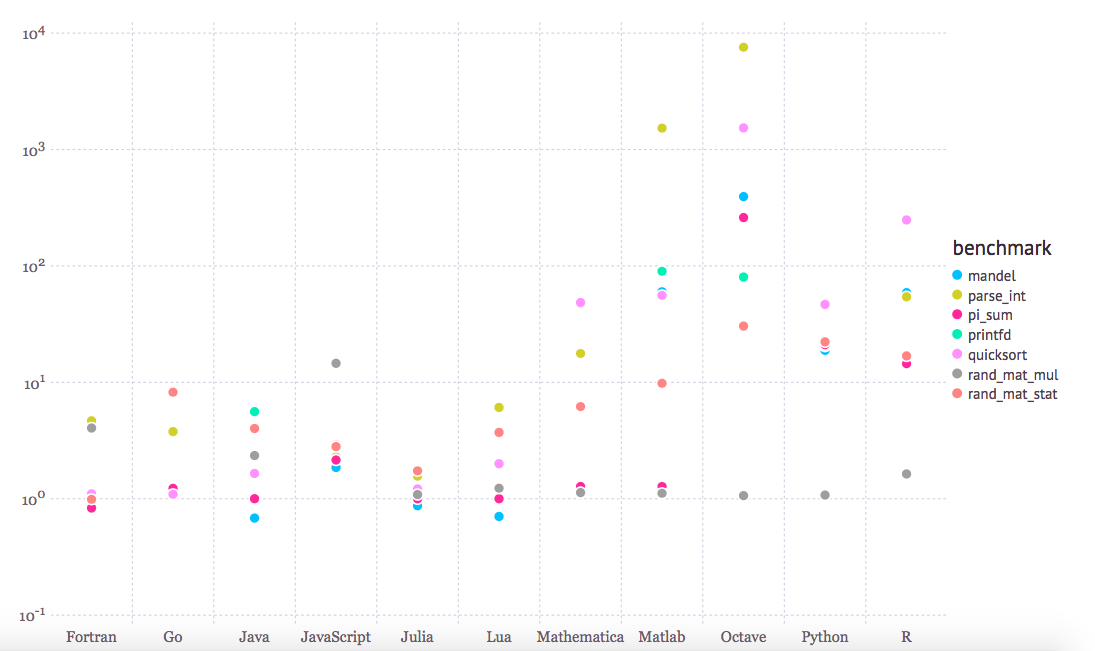
\includegraphics[width=0.95\textwidth]{images/julia_benchmark.png}
\label{bench}
\caption{Comparison of performance for several computing languages. Benchmark times relative to C (smaller is better, C performance = 1.0). Source: https://julialang.org/benchmarks/.}
\end{figure}


There are more specialized languages, such as R, Julia. But we will try to keep the things simple here by showing how the same task is programmed in the 3 languages we have selected.
See for example \ref{bench} for a comparison on the performance of those different languages.

I am taking these examples from http://rosettacode.org.
To give you a flavor of what is the feeling writing code in those 3 languages I have selected 2 tasks and showing how the solution is express in those languages.

\subsection{Sieve of Eratosthenes}

The Sieve of Eratosthenes is a simple algorithm that finds the prime numbers up to a given integer.

Lets start with the implementation in C. I am selecting not the most optimized version, but the simplest implementation for pedagogical purposes. The idea is to get a flavor of the language.

\lstinputlisting[language=C]{../Day3_AdvancedTopics/2.Programming/sieve.c}

This example shows the basic elements from the c language, the creation of variables, loops and conditionals. The inclusion of libraries and the printing on screen.

You can compile this code using the code at 

\begin{lstlisting}
Day3_AdvancedTopics/2.Programming
\end{lstlisting}

\begin{lstlisting}
gcc sieve.c -o sieve
\end{lstlisting}

and execute like this

\begin{lstlisting}
./sieve 100
\end{lstlisting}

Now lets consider the Fortran version of the same problem.

\lstinputlisting[language=Fortran]{../Day3_AdvancedTopics/2.Programming/sieve.f90}

You can notice the particular differences of this language compared with C, working with arrays is in general easier with Fortran.

You can compile this code using the code at 

\begin{lstlisting}
Day3_AdvancedTopics/2.Programming
\end{lstlisting}

\begin{lstlisting}
gfortran sieve.f90 -o sieve
\end{lstlisting}

and execute like this

\begin{lstlisting}
./sieve 100
\end{lstlisting}

Finally, this is the version of the Sieve written in python

\lstinputlisting[language=Fortran]{../Day3_AdvancedTopics/2.Programming/sieve.py}

Python is an interpreted language so you do not need to compile it, instead directly execute the code at:

\begin{lstlisting}
Day3_AdvancedTopics/2.Programming
\end{lstlisting}

using the command line:

\begin{lstlisting}
python sieve.py 100
\end{lstlisting}


%\begin{lstlisting}[language=Python, numbers=left]
%import numpy as np
%def incmatrix(genl1,genl2):
%    m = len(genl1)
%    n = len(genl2)
%    M = None #to become the incidence matrix
%    VT = np.zeros((n*m,1), int)  #dummy variable
% 
%    #compute the bitwise xor matrix
%    M1 = bitxormatrix(genl1)
%    M2 = np.triu(bitxormatrix(genl2),1) 
% 
%    for i in range(m-1):
%        for j in range(i+1, m):
%            [r,c] = np.where(M2 == M1[i,j])
%            for k in range(len(r)):
%                VT[(i)*n + r[k]] = 1;
%                VT[(i)*n + c[k]] = 1;
%                VT[(j)*n + r[k]] = 1;
%                VT[(j)*n + c[k]] = 1;
% 
%                if M is None:
%                    M = np.copy(VT)
%                else:
%                    M = np.concatenate((M, VT), 1)
% 
%                VT = np.zeros((n*m,1), int)
% 
%    return M
%\end{lstlisting}


\section{Introduction to Parallel Programming}

Parallel programming is essential in High-Performance Computing. Computers nowadays are not increasing speed as they use to years ago.
Instead, they increase the number of cores.
Modern HPC clusters are now build from several nodes, with several processors each and with several cores each processor.
Those processing capabilities are complemented by adding GPU and Co-processors such as Xeon Phi.

For this tutorial we will consider two popular alternatives for parallel computing, both OpenMP and MPI offers ways of execute calculations concurrently on several cores.
An application can run on a computer cluster using both OpenMP and Message Passing Interface (MPI), such that OpenMP is used for parallelism within a (multi-core) node while MPI is used for parallelism between nodes.

We will explore those two kinds of parallel programming alternatives with a few examples each.

\section{Parallel Programming with OpenMP}

OpenMP (Open Multi-Processing) is an application programming interface (API) that supports multi-platform shared memory multiprocessing programming in C, C++, and Fortran.

The basic idea is to write special comments called ``pragmas" that will be interpreted by the compiler when you compile the code with some special argument. In most cases the code can compile just fine without the extra argument and it will work as a serial code, using just one core.

Lets start with the usual hello program. This is the implementation in C 

\lstinputlisting[language=C]{../Day3_AdvancedTopics/4.OpenMP/omp_hello.c}

You compile it with the command

\begin{lstlisting}
gcc -fopenmp omp_hello.c -o hello
\end{lstlisting}

The version in Fortran is:

\lstinputlisting[language=C]{../Day3_AdvancedTopics/4.OpenMP/omp_hello.f90}

You compile it with the command

\begin{lstlisting}
gcc -fopenmp omp_hello.f90 -o hello
\end{lstlisting}

When you execute the program you will see messages comming from the different threads, all the program runs on the same machine but it creates threads to concurrently execute the section enclosed by the \verb|"#pragma"| or \verb|"!$omp"|
blocks.

You can control the number of threads using

\begin{lstlisting}
export OMP_NUM_THREADS=3
\end{lstlisting}


\section{Parallel Programming with MPI}


\section{Test Driven Development}


\section{Version control with Git}

The tutorial about Git will be based on the repository created at:

\begin{lstlisting}
https://github.com/guilleaf/TutorialGitAutotools
\end{lstlisting}


%\section{Optimization, Profiling and Debugging}

%\section{Creating Python Modules}
%\section{Continuous Integration}


\end{document}
